%%%%%%%%%%%%%%%%%%%%%%%%%%%
% Do Elections Affect Fed Forecasts?
% Cassandra Grafström and Christopher Gandrud
% 8 April 2013
%%%%%%%%%%%%%%%%%%%%%%%%%%%%

% !Rnw weave = knitr

\documentclass[a4paper]{article}
\usepackage{fullpage}
\usepackage[authoryear]{natbib}
\usepackage{setspace}
    \doublespacing
\usepackage[usenames,dvipsnames]{xcolor}
\usepackage{hyperref}
\hypersetup{
    colorlinks,
    citecolor=black,
    filecolor=black,
    linkcolor=cyan,
    urlcolor=cyan
}
\usepackage{dcolumn}
\usepackage{booktabs}
\usepackage{url}
\usepackage{tikz}
\usepackage{todonotes}
\usepackage[utf8]{inputenc} 

% Set knitr global options



%%%%%%% Title Page %%%%%%%%%%%%%%%%%%%%%%%%%%%%%%%%%%%%%%%%%%%%
\title{Inflated Expectations: How government partisanship shapes bureaucrat's inflation expectations}

\author{Christopher Gandrud \\
                {\emph{Yonsei University}}\footnote{\href{mailto:gandrud@yonsei.ac.kr}{gandrud@yonsei.ac.kr}} \\
                and \\
            Cassandra Grafstr\"{o}m \\
                {\emph{Hertie School of Governance \& University of Michigan}}\footnote{\href{mailto:cgrafstr@umich.edu}{cgrafstr@umich.edu}}}

\begin{document}

\maketitle

%%%%%%% Abstract %%%%%%%%%%%%%%%%%%%%%%%%%%%%%%%%%%%%%%%%%%%%
\begin{abstract}
\noindent\emph{Working draft. Comments welcome.}\footnote{Thank you to the Mark Hallerberg and the Fiscal Governance Centre at the Hertie School of Governance for comments and support. Thank you also to Leonardo Baccini, Vincent Arel-Bundock, Cheryl Schonhardt-Bailey, Tom Stark, and seminar participants at the Hertie School of Governance, London School of Economics, and Yonsei University. \\
This paper was written using {\tt{knitr}} \citep{knitr2013}. It can be entirely replicated from data, analysis source code, and markup files available on our GitHub page at: {\url{https://github.com/christophergandrud/GreenBook}}.} \\[0.2cm]


A government's party identification can indicate the types of economic policies that it is likely to pursue. Left-party governments are expected to pursue policies that promote lower unemployment, but which may cause inflation. Right party governments are expected to pursue lower inflation policies. How do these expectations shape monetary policy bureaucrat's inflation forecasts? If there is a mismatch between the policies bureaucrat's \emph{expect} governments to implement and those that they \emph{actually} do, forecasts will be systematically biased. There is evidence that at least in the United States the real differences in policies implemented by left-leaning Democratic and right-leaning Republican presidents is minimal \citep{Bartels2008}. Using Fed staff's Greenbook forecasts we test for presidential partisan biases. We find that irrespective of actual policy and economic conditions forecasters \emph{do} systematically overestimate inflation during Democratic presidencies and underestimate inflation during Republican ones. Our findings suggest that Fed staff's inflation forecasts are shaped by heuristic presidential partisan biases.

\end{abstract}

\begin{description}
  \item [{\textbf{Keywords:}}] forecast bias, Federal Reserve bureaucrats, rational partisan cycle, heuristics, inflation, monetary policy
\end{description}

\vspace{0.3cm}


Monetary policy is an inherently forward looking enterprise. Beliefs about the economy's future course guide the setting of interest rates. Government policies significantly affect changes in growth, inflation, and unemployment. A government's party identification can serve as a cue for the types of economic policies that it is likely to pursue during its tenure. In the United States, Republicans are expected to pursue policies associated with lower inflation and Democrats are expected to pursue policies associated with lower unemployment, but more inflation. Evidence suggests, however, that the real differences in policies implemented by the two parties is quite minimal \citep{Bartels2008}. How do US Federal Reserve staff incorporate the government's partisan composition when forming expectations of future inflation?

There is an extensive literature looking for partisan effects in monetary policy-makers' choices. This literature is divided into two broad groups. One group has examined how monetary policymakers--in the US the Federal Open Markets Committee (FOMC)--may use interest rates to advantage incumbents they support and harm those they do not \citep{Clark2012,Hakes1988,Sieg1997,Tootell1996}. The second group--the rational partisan expectations literature--has assumed that policymakers do not prefer one part over the other, but choose monetary policies to control inflation given their expectations about what policies different governments will pursue \citep{Alesina1991,Hibbs1994}. We add to the understanding of monetary policymaking by taking a step back, examining how government partisanship shapes the bureaucratic inflation forecasts that influence policymakers' choices.

We provide evidence that Fed internal inflation forecasts consistently predict that inflation will be lower than it turns out to be under Republican presidencies and predict that inflation will be higher than it turns out to be under Democratic administrations. Even accounting for changes in monetary policy and a variety of other economic and political factors, Federal Reserve economists over-shoot inflation forecasts for Democrats and under-shoot for Republicans. We find evidence that rather than partisan preferences or rational monetary policy expectations the use of partisan heuristics by Fed staffers explains these predictive failures.

In this paper we first briefly describe bureaucratic inflation forecasting at the US Federal Reserve and why it is important for monetary policymaking. Then we introduce competing hypothesis about how partisan control of the presidency might shape inflation forecasts by the Federal Reserve staff. We then define what inflation forecast errors are. We demonstrate in this section using Fed Staff's ``Greenbook'' forecasts that there does appear to be a partisan bias. Up until now academic scholarship has not examined this bias. We test the theories of partisan bias with a series of regression models using both unmatched and matched data on Greenbook inflation forecast errors from the 1970s through 2007.\footnote{This is the most complete data set currently available to the public.} Our findings suggest that even when controlling for a number of important economic and political factors, Greenbook forecasts show a distinct presidential partisan bias across presidential terms. Rather than being caused by electoral preferences or partisan monetary policy expectations, causes previously addressed in the monetary policy literature, we find evidence that the bias is caused by an incorrect partisan heuristic Fed staff have about administrations' likely affect on inflation. In the conclusion we discuss the implications of these findings for monetary policy and election outcomes and future directions for research.

%%%%%%%%%%%%%% Section 1: Forecasting Inflation at the Fed %%%%%%%%%%%%%%%%%%%%%

\section{Bureaucratic Inflation Forecasting in the United States}

The US Federal Reserves Greenbook forecasts are an important example of bureaucratic inflation forecasting. Prior to every FOMC meeting Federal Reserve staff create a document called the ``Current Economic and Financial Conditions"--Greenbook--that contains information on recent behavior and forecasts of various macroeconomic aggregates assuming no monetary policy change.\footnote{Greenbook data can be found at {\url{http://www.phil.frb.org/research-and-data/real-time-center/greenbook-data/philadelphia-data-set.cfm}} (accessed March 2013). Greenbook forecasts are currently available to the public for each quarter from the fourth quarter of 1965 through the end of 2007. There is a five year lagged release schedule. Also, some forecasts are not available for the entire period.} Federal Reserve staff make forecasts of various elements of the US and global economies so that the FOMC can make policies appropriate to fulfill the Fed's dual mandate of maintaining maximum employment and price stability. 

As \cite{Svensson2005} notes, the accuracy of forecasts is essential to the effectiveness of monetary policy. The FOMC uses these forecasts to determine the appropriate monetary policy to pursue. Higher inflationary expectations increase the likelihood of the FOMC tightening policy in order to slow inflation and an overheating economy; low inflationary expectations increase the likelihood of a loosening of monetary policy to bolster growth and employment, all else equal. Therefore, it is important that Greenbook forecasts accurately predict future inflation.

The study of Fed inflation forecasts and their accuracy has been almost exclusively contained within economics with the main concern being the rationality of forecasts \cite[e.g.][]{Capistran2006, Romer2000} and the performance of the Fed's forecasts relative to market forecasts \cite[e.g.][]{Faust2007, Gamber2009}. While some studies have examined the biases of particular time periods \cite[e.g.][]{Capistran2006} or bank presidents \cite[e.g.][]{Havrilesky1995}, in our search none considered how government partisanship affects expectations about future inflation.
 
While the idea that politicians of different partisan stripes might behave differently in office and that their behavior might have different effects on future economic output and inflation is largely uncontroversial,\footnote{See \cite{Bartels2008} for evidence on the similarities and differences of Democrats and Republicans in office.} there have been no tests of whether or how these differences would affect inflation forecasts. It is important to note that finalized Greenbook forecasts are ``consensus" forecasts combining \textbf{both} econometric models and the professional opinions of forecasters about likely changes in the economy's trajectory not necessarily picked up in these models \citep{Karamouzis1989,Reifschneider1997}. Preferences and/or beliefs about government partisanship could therefore directly shape Greenbook forecasts.

%%%%%%%%%%%%%%%%%%%%%%%%%%%%% Section 2: Possible Explanations of Fed Inflation Forecast (In)accuracy %%%%%%%%%
\section{Possible Explanations of Fed Inflation Forecast Inaccuracy}

In this section we try understand Fed bureaucrat's inflation forecast accuracy by developing theories derived from the political economy and political psychology literatures that provide possible explanations of how government partisanship may shape forecasts. 

\subsection{Econometric Models \& Accuracy}

Before digging into partisan explanations of forecast errors, which would largely be the result of Federal Reserve staff judgment, it is worth examining the possibility that forecast inaccuracy is the result of systematic errors in the staff's predictive econometric models. Federal Reserve staff have used two primary sets of econometric models during the period for which Greenbook data is available.\footnote{This subsection draws heavily on Brayton et al.'s \citeyear{Brayton1997} detailed description of the changes to Federal Reserve forecasting models that took place in 1996.} 

The first simultaneous equation model of the US and world economies were developed and adopted by the Federal Reserve between 1966 and 1975. This model was based on adaptive expectations and largely extrapolated future behavior of the economy from its recent past behavior. New models of the American and world economies' near-term trajectories were introduced in the 1990s, fully replacing the older model in 1996. The Federal Reserve Board US model (FRB/US) explicitly considers the role of economic expectations in economic behavior. The foundational assumption of adaptive expectations in the old model was replaced with rational or model-consistent expectations. In these models, prices are sticky and aggregate demand determines short-run output. Furthermore, monetary policy's effects on the economy are extensively modeled. 

Presumably, the move to rational expectations would improve forecast accuracy relative to the earlier period. The goal of incorporating forward looking actors into the models was to account for an important source of endogeneity in earlier models that could lead to overestimates of important economic indicators under some circumstances and underestimates of those same indicators under others. None of these over or underestimates, however, ought to have been linked to the party of the president. We would, however, expect that the \emph{magnitude} of forecast errors changed after 1996.

\subsection{Partisan Biases \& Accuracy}

There is an extensive literature looking for partisan effects in monetary policy, but no studies examining the impact of presidential partisanship on predictions of inflation. Studies have looked for evidence of partisan preferences manifesting themselves in the monetary policies chosen by the FOMC. There are two essential reasons that partisan effects would be found in policy: either a preference for one party over another by members of the FOMC or an expectation that once in office the parties will engage in systematically different policies that will influence inflation, leading the FOMC to support more preferred policies and attempt to inhibit less preferred ones. 

The preference arguments assume that a conservative central banker will prefer the election of politicians who hold more similar inflationary preferences (i.e., those with a stronger preference for low inflation) and enact policies to bolster their preferred candidate's prospects of being elected. In the US this would mean that the Federal Reserve would implement policies that supported the electoral prospects of Republican incumbents and harm the electoral prospects of Democratic incumbents \citep{Clark2012,Hakes1988,Sieg1997,Tootell1996}.

The rational partisan expectations literature assumes that central bankers do not have an innate preference for one party over another, but instead expect Democrats and Republicans to behave differently in office \citep{Alesina1991,Hibbs1994}. It is these behavioral expectations that would lead to different monetary policies under Democratic and Republican presidencies, with the former expected to engage in more expansionary and inflationary policies than the latter. In order to stave off higher inflation under a Democrat the Fed would tighten monetary policy; because Republicans are expected to prefer low inflation, they will pursue low inflation policies and so the FOMC can accommodate Republican presidents' policies without fear of stoking inflation. This argument is again based on the assumed preferences of partisans, but does not require the FOMC to be politically biased as the former does. 

Arguments similar to those in the literature on partisan monetary cycles can be adapted to predict patterns of partisan differences in inflation forecasts. We present three theoretical arguments about how inflation expectations would differ by the President's party: the partisan preference theory, the monetary expectations theory, and the partisan heuristics theory (see Figure \ref{ExpectGraphs} for an illustration of the theories' contrasting inflation error predictions).





% Define colors for figure
%% See: http://colorbrewer2.org/
\definecolor{DEM}{HTML}{2259B3}
\definecolor{REP}{HTML}{C42B00}

\begin{figure}
  \caption{Stylized Partisan Inflation Forecast Error Predictions}
  \label{ExpectGraphs}
  \begin{center}

    \vspace{0.25cm}

    \tikzstyle{bagMain} = [text width = 5cm]
    \tikzstyle{bagDem} = [text = DEM]
    \tikzstyle{bagRep} = [text = REP]
    
    \tikzstyle{DemLine} = [draw, 
                          color=DEM,
                          opacity=0.9,
                          line width=1.5mm]

    \tikzstyle{RepLine} = [draw, 
                          color=REP,
                          opacity=0.9,
                          line width=1.5mm]

\begin{tikzpicture}

  %%%% Partisan Preferences
  \node (PP) at (-7, 5) [bagMain]{{\bf{Partisan Preferences}}};
  \node (E) at (-10.5, 3.25) [bagMain, rotate=90]{{\emph{Forecast Error}}};
  \node (T) at (-7.3, -0.5) [bagMain]{{\emph{Duration of Pres. Term}}};
  
  \draw (-10, 0) -- (-6, 0);
  \draw (-10, 0) -- (-10, 4);
  
  \draw[RepLine] (-9.5, 1.9) -- (-7.5, 1.9); 
  \draw[DemLine] (-9.5, 2.1) -- (-7.5, 2.1); 

  \draw[RepLine] (-7.52, 1.9) -- (-6.5, 1); 
  \draw[DemLine] (-7.52, 2.1) -- (-6.5, 3); 

  \node (R1) at (-6.5, 0.5) [bagRep]{Rep.};
  \node (D1) at (-6.5, 3.5) [bagDem]{Dem.};

  
  %%%% Monetary Expectations
  \node (PP) at (-2, 5) [bagMain]{{\bf{Monetary Expectations}}};
  
  \draw (-5, 0) -- (-1, 0);
  \draw (-5, 0) -- (-5, 4);
  
  \draw[RepLine] (-4.5, 2.1) -- (-2.5, 2.1); 
  \draw[DemLine] (-4.5, 1.9) -- (-2.5, 1.9); 

  \draw[DemLine] (-2.52, 1.9) -- (-1.5, 1); 
  \draw[RepLine] (-2.52, 2.1) -- (-1.5, 3); 

  \node (D2) at (-1.5, 0.5) [bagDem]{Dem.};
  \node (R2) at (-1.5, 3.5) [bagRep]{Rep.};
  
  
  %%%% Partisan Heuristics
  
  \node (PP) at (3, 5) [bagMain]{{\bf{Partisan Heuristics}}};
  
  \draw (0, 0) -- (4, 0);
  \draw (0, 0) -- (0, 4);
  
  \draw[DemLine] (0.5, 3) -- (4, 3); 
  \draw[RepLine] (0.5, 1) -- (4, 1); 

  \node (D3) at (3.5, 3.5) [bagDem]{Dem.};
  \node (R3) at (3.5, 0.5) [bagRep]{Rep.};

  \end{tikzpicture}
  \end{center}
\end{figure}





The {\bf{partisan preference theory}} of inflation forecast errors is similar to the partisan preference model of monetary policy described above. This theory assumes that Fed staff have a preference for more inflation averse politicians to control the executive and so produce inflation forecasts that would justify the implementation of easy monetary policy under Republican administrations and tight money under Democratic administrations, particularly as presidential elections approach. The FOMC, choosing policy based on these forecasts would then implement monetary policies to optimize its utility function, which would not need to depend upon presidential partisanship at the level of the FOMC. However, because Fed staffers prefer low inflation to high, they would not necessarily want to produce too loose/tight monetary policy over an entire four year term. Instead, they would want to encourage an economic boost (contraction) near the end of a Republican (Democratic) presidency. This implies that realized inflation would be higher than forecasted during Republican presidencies and lower than forecasted for Democratic presidencies. These effects would be particularly pronounced in the {\emph{quarters running-up to elections}} as Fed staff attempt to help their favored political party \citep{Beck1987,Grier1987}. Further, accounting for actual changes in monetary policy ought to increase the magnitude of partisan effects. This is because predictions of inflation during Republican presidencies, for example, will be lower than what the staff actually expects. If looser monetary policy is implemented in response to these low inflation forecasts than would have been chosen under the staff's true inflationary expectations, inflation will actually be higher than the staff's original forecast.

What we call the {\bf{monetary expectations theory}} is based on an assumption of partisan bias in the FOMC. It assumes that Federal Reserve economists believe members of the FOMC will engage in partisan monetary policy by lowering interest rates under conservative administrations and increasing them under liberal presidents, as \cite{Clark2012} found, and that the FOMC is doing this to manipulate election outcomes. In this formulation, the Fed staff has no preference for one party over another, but knows that the FOMC does and so formulates estimates in order to counter the FOMC's policies. If Fed economists believe that the Open Market Committee will choose systematically higher-than-called-for interest rates during Democratic presidencies and vice versa for Republicans, then--assuming they are interested in the implementation of optimal monetary policies--they would produce forecasts that are higher than expected during Republican administrations and the lower for Democrats; the {\emph{opposite of what is expected in the partisan preference theory}}. If the FOMC fails to note the compensation made by the Fed staff, then we would expect that after accounting for implemented policies inflation forecasts would be higher than or equal to realized inflation during Republican terms and lower than or equal to forecasts under Democratic administrations.\footnote{This is the formulation of the monetary expectations theory illustrated in the center panel of Figure \ref{ExpectGraphs}.} If, however, the FOMC anticipated these compensatory biases in staff forecasts, then the FOMC would discount the Greenbook estimates and continue to implement inflationary policies during Republican administrations and contractionary policies during Democratic ones. If the staff likewise know that they are not being listened to they may randomize their errors, producing an uninformative signal \citep{Crawford1982}. This would result in approximately similar inflation forecast errors for both Republicans and Democrats. However, we largely did not observe this and it is not illustrated above. If the Fed staff believes that the FOMC will engage in this behavior only when presidential elections are approaching, then we would expect no partisan differences in forecasts at the beginning of a presidency but increasing divergence as the term wanes.
 
The {\bf{partisan heuristics theory}} proposes that Fed staffers incorporate a heuristic \citep[see][]{kahneman1973, tverskykahneman1974, kahneman2003} about the policy behaviors of presidents from different parties and the effects these different policies will have on the economy. Heuristics are intuitions that reduce the complexity associated with making predictions. Though they can be useful ``sometimes they lead to severe and systematic errors" \citep[][1124]{tverskykahneman1974}. In this theory, economists at the Fed have an intuition that Democrats and Republicans behave differently in government and so formulate inflationary expectations with this in mind. If this intuition does not accurately correspond to how presidents act, or how their policies impact inflation, forecasts will be systematically biased: overestimates for Democratic presidents, underestimates for Republicans. \cite{Bartels2008} finds evidence that Democratic and Republican presidents do not, in fact, differ significantly in their overall levels of spending, so any expectation that they would pursue policies that would differentially affect inflation in the medium-run would be inaccurate.\footnote{\cite{Bartels2008} does not discuss other policies that could affect inflation in the long run, such as changes to labor and financial market regulation. These policies too would be expected to differ by party, however their lags are likely to be quite long and out of the forecasted time frames used in this paper.} These biases should be constant {\emph{across presidential terms}}, in contrast to the partisan preference and monetary expectation theories, which both assume an intensification of biased behavior as elections approach.

This model does not require that forecasters be conscious of the heuristics they're using, but simply for it to work its way subtly into forecasts, particularly in the subjective aspect of the ``consensus forecast" component of the Greenbook. Further, because this bias would not need to be conscious, the systematic error could easily go unnoticed (as mistakes could occur for any number of idiosyncratic or economic reasons). If the bias goes unnoticed, then it will not be corrected in future inflation predictions. This differs from the rational partisan expectations theory described above in the monetary policy outcome literature in two ways. First, because these beliefs are not updated to account for the lack of partisan differences in spending they are not ``rational". Second, and relatedly, this theory is based on psychological instead of game theoretic reasoning, which allows for the persistence of suboptimal strategies in a way that would be less likely in a rational choice model of this same process given the assumption that the goals of the actors are the same in the two models. 

%%%%%%%%%%%%%%%%%% Section 3: Forecast Accuracy %%%%%%%%%%%%%%%%%%
\section{Federal Reserve Staff's Forecast Accuracy}\label{ForecastAcc}

How accurate are Fed staff forecasts? We focus on Greenbook forecasts of the GNP/GDP price index forecasts. We choose this indicator of Federal Reserve forecast accuracy both because there is a strong theoretical assumption that central bankers are more inflation averse than politicians \citep[e.g.][]{Cukierman1992,Mukherjee2008,Tillmann2008} and because this is the dominant measure of forecast errors used in the economics literature \citep[c.f.][]{Romer2000}. We measure accuracy by calculating {\bf{forecast error}} $E$ as the difference between the Greenbook inflation forecast $F$ for a given quarter $q$ and actual inflation $I$ as a proportion of actual inflation:
%
\begin{equation}
    E_{q} = \frac{F_{q} - I_{q}}{I_{q}}.
\end{equation}
%
We choose to focus on proportional rather than absolute errors\footnote{Absolute errors are: $F_{q} - I_{q}$.} because it is substantively more meaningful for comparing errors across time periods. As shown in Figure \ref{absolute}, absolute inflation varies considerably across different periods. To be able to easily estimate meaningful effects on errors across time we need to look at proportional rather than absolute errors.\footnote{Note that the direction and significance of our main findings do not change when we use absolute rather than proportional errors in our estimation models (discussed below). The magnitude does change, but this is to be expected because the range of the absolute inflation errors is much larger than proportional errors. These results are available from the authors upon request.}

If the forecasts are unbiased the mean error of the forecasts would be indistinguishable from zero. While \cite{Romer2000} found that the Fed's internal forecasts  meet this requirement over the full history of Greenbook forecasts, such an amalgamation disguises long periods of over- or under-predicting inflation, as noted in \cite{Capistran2006} and illustrated in Figure \ref{absolute}. Within economics the Fed's forecasts have been examined for evidence of rationality. These studies generally find that the Fed rationally incorporates information into its forecasts, outperforming private forecasts \cite[c.f.][]{Gamber2009}. These studies, however, have rarely incorporated Fed staff member' political preferences, because Federal Reserve staffers are assumed to be politically independent.

Our dataset has 169 forecast quarters, spanning the fourth quarter of 1965 through the end of 2007. Greenbook forecasts correspond to those provided for the FOMC meeting closest to the middle of the quarter. We found actual inflation corresponding to each of these quarters\footnote{Inflation was calculated by comparing quarters year-on-year. The exact inflation measure that the Federal Reserve was forecasting changed a number of times, so the measure of actual inflation used to created the forecast error variable changes accordingly. The GNP deflator indicator is used from the beginning of our sample through the end of 1991. From the first quarter of 1992 through the first quarter of 1996 actual inflation is measured with the GDP deflator. From the second quarter of 1996 we use the chain-weighted GDP price index. For more details on how the forecasted quantity changed see the Greenbook data description file available at: \url{http://www.phil.frb.org/research-and-data/real-time-center/greenbook-data/philadelphia-data-set.cfm}. The Greenbook inflation forecast variable we used is called ``PGDPdot''.} using data from the Federal Reserve's FRED website.\footnote{See \url{http://research.stlouisfed.org/fred2/}. Accessed December 2011.} We examine errors made by forecasters in the current quarter and all quarters up to five quarters before.\footnote{The Greenbook contains very incomplete data for forecasts made over longer time spans.} The results are generally the same regardless of the forecast used, especially the presidential partisan findings (see Figure \ref{ExpectValueParty}). For simplicity, the majority of results we show and discuss in detail are from models with forecasts made two quarters beforehand.\footnote{Using these two quarter forecasts restricts our observations because they are rarely available before the 1970s.} Figure \ref{absolute} compares absolute actual inflation for each quarter and inflation forecasts made two quarters before.

%%%%%%%%%%%%%%%%%%%%%%%%%%  Raw Greenbook estimate vs. actual graph
\begin{figure}[t]
    \caption{Greenbook Inflation Forecasts Made 2 Qtr. Beforehand and Actual Quarterly Inflation}
    \label{absolute}
    \begin{center}
    
\begin{knitrout}
\definecolor{shadecolor}{rgb}{0.969, 0.969, 0.969}\color{fgcolor}

{\centering 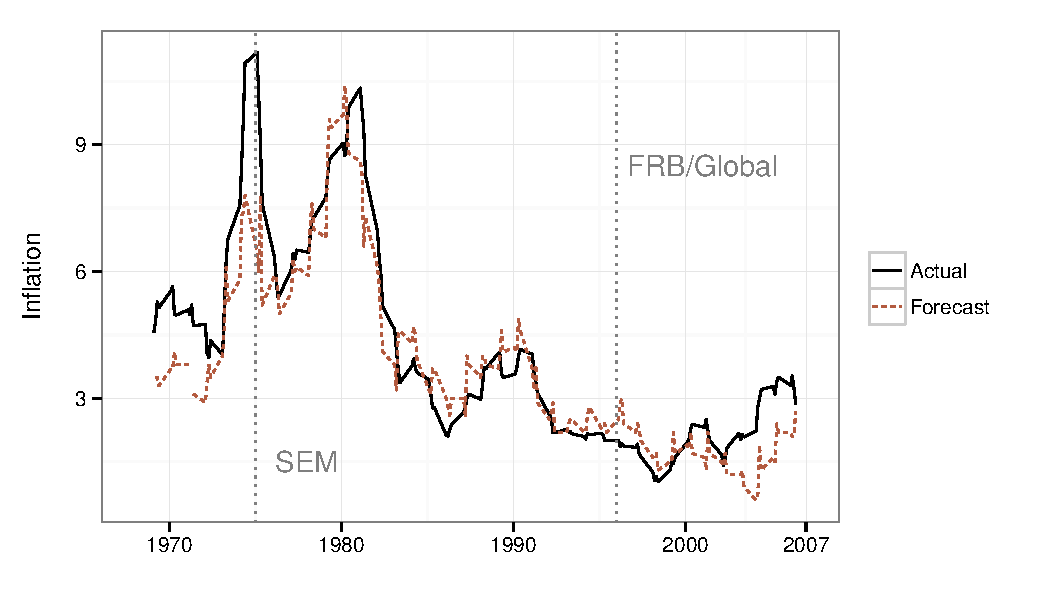
\includegraphics[width=0.8\linewidth]{figure/BaseInflation} 

}



\end{knitrout}

    
    \end{center}
    \begin{singlespace}
        {\scriptsize{The vertical grey dotted line indicates when the Federal Reserve Board Global (FRB/Global) forecasting model was fully implemented.  
                      }}
    \end{singlespace}
\end{figure}


\subsection{Are There Partisan Forecast Errors?}




Unbiased forecasts have a mean error of zero \citep[5]{Bruck2006}. Using this criteria, forecast errors should be the same--ideally with a mean of 0--regardless of the incumbent president's party identification. This is not the case. From the second quarter of 1969\footnote{Data availability for two quarter forecasts before 1969 is lacking.} through 2007 the mean standardized forecast error was -0.04, i.e. forecasters under-predicted inflation by about 4 percent. The mean error is noticably different across Republican compared to Democratic presidencies. Across Republican presidencies it was -11 percent and 13 percent across Democratic presidencies.\footnote{These means are from estimates made two quarters beforehand. Both means are statistically significantly different from 0, the full observation mean, and each other at the 99\% confidence level. For more details see \url{http://bit.ly/WHsRYh}.} On average, inflation was underestimated in Republican presidencies and overestimated in Democratic ones.

Figure \ref{errors_over_time} plots forecast errors across our sample separated by presidential term and party. The first thing to note is that inflation was rarely underestimated during the three Democratic presidential terms in our sample. The underestimates that were made were relatively small. The largest overestimates we see were made during Bill Clinton's (Democratic) presidency. All of the major inflation underestimates were made during Republican presidencies, particularly during Richard Nixon's, Gerald Ford's, and George W. Bush's presidencies. Inflation was often overestimated during the second part of Reagan's first term, his second term and George H.W. Bush's term. Over this period--often referred to as the Volcker Revolution \citep{Bartels1985}--inflation was suddenly much lower than before (see Figure \ref{absolute}). It may have taken awhile for forecasters to adjust to this new lower level of inflation, particularly because the Fed's own models of the economy assumed that money had no real effects on the economy during this period, even while the FOMC was pursuing aggressive anti-inflation policies.

This summary examination of inflation forecast errors suggests that there may be a presidential partisan bias. What might explain this?

%%%%%%%%%%%%%%%%%%%%%%%%%%   Greenbook Error Across Time
\begin{figure}[t]
    \caption{Errors in Inflation Forecasts Made 2 Qtr. Beforehand (1969 - 2007)}
    \label{errors_over_time}
    \begin{center}
    
\begin{knitrout}
\definecolor{shadecolor}{rgb}{0.969, 0.969, 0.969}\color{fgcolor}

{\centering \includegraphics[width=0.8\linewidth]{figure/PartisanError} 

}



\end{knitrout}

    
    \end{center}
    \begin{singlespace}
        {\scriptsize{Note: An error of 0 indicates that inflation was perfectly predicted.}}
    \end{singlespace}
\end{figure}



%%%%%%%%%%%%%%%%%% Section 4: Research Methods %%%%%%%%%%%%%%%%%%

\section{Research Methods}

We use non-matched and matched data sets with parametric models \citep[see][]{Ho2007} to assess whether and what types of partisan biases exist in Greenbook inflation forecasts. This section discusses the choice of methods and variables. In the following section we discuss our results.

\subsection{Matching}

We are interested in disentangling the effects of presidential party ID and elections from many background factors, such as economic shocks and FOMC policy changes, that would create inflation forecast errors. As such, we consider presidential partisan identification and elections to be `treatments' that may impact inflation forecast errors. Democratic presidencies are considered to be treatments. Republican presidencies are `controls'.\footnote{The selection of `treatment' and `control' groups in this context is arbitrary.} Quarters when a presidential election is held and the quarter before it are considered treatments and all other quarters are controls. Of course, given that we are working with observational data, other variables that have an impact on forecast errors may have {\emph{different distributions}} across the treatment and control groups \citep{Cochran1973, Diamond2012}. This makes it difficult to identify the relationships between presidential party ID, elections and errors from all of the confounding background variables.

To address this issue we follow the advice of \cite{Ho2007} to pre-process data with matching to create data sets where the distributions of confounding variables are more even across treatment and control groups. We then run parametric analyses with the matched data sets. We use the {\tt{R}} package {\tt{MatchIt}} \citep{matchit2011} to create two matched data sets where the non-treatment covariates in the control groups closely match those in the treatment groups. Doing this helps us isolate the effects of the `treatments' from that of the background covariates by producing a data set of control and treatment units with the same distribution of the covariates \citep{matchit2011}. This is known as ``covariate balance" \cite[1]{Diamond2012}. Using matching to balance a data set ``break[s] the link between the treatment variables and the pre-treatment controls", effectively replicating the conditions of a randomized experiment with observational data \cite[][2--3]{matchit2011}. 

Balance is usually achieved in matching through propensity scores: the probabilities that units were assigned the treatment given their covariates. The propensity score model is generally unknown \citep{Drake1993}. To find the propensity score model we use Diamond and Sekhon's \citeyearpar{Diamond2012} genetic matching method (GenMatch).\footnote{The method is implemented with {\tt{MatchIt}}. The original source code for our exact matching models can be found at {\url{http://bit.ly/OFdA4u}}.} GenMatch is a multivariate method that uses an evolutionary search algorithm to automate the search for the propensity score model that creates maximum balance. This minimizes the difficulty of ``manually and iteratively checking the propensity score" to determine covariate balance \citep[][2]{Diamond2012}. 


\subsection{Parametric Models}

Once we created our matched data sets we used two types of parametric models to examine the effects of our treatment variables on the continuous inflation forecast error variable.\footnote{Parametric models are estimated using the \texttt{R} package \texttt{Zelig} \citep{Zelig2012}.} The first was normal linear regression using maximum likelihood estimation of variance.\footnote{In {\tt{Zelig}} this is the {\tt{normal}} model. We also used ordinary least squares (in \texttt{Zelig}, this is the \texttt{ls} model). The results were virtually identical.} The other type was Bayesian normal linear regression\footnote{In {\tt{Zelig}} this is the {\tt{normal.bayes}} model. Bayesian normal linear regression is particularly useful for our limited sample as it makes ``valid small sample inferences via draws from the exact posterior" \citep[][38]{Zelig2012}. Please see \cite{Goodrich2007} for details about Bayesian normal linear regression.  See also \cite{Imai2008} for a discussion of how to combine non-parametric matching and parametric analysis in one research process.} Because we used  matching methods, not only do we better isolate the treatments' effects from those of the background variables, but we also reduce our estimated causal effects' dependence on the type of model we choose \cite[200--201]{Ho2007}.

The generic parametric models we used is given by
%
\begin{equation}
    E_{q} = \alpha + \beta_{T} T_{q} + \beta_{X} X_{q} + \epsilon,
\end{equation}
%
where $T$ is the treatment and $X$ is a vector of covariates. 

\subsection{Variables}

In Section \ref{ForecastAcc} we discussed our dependent variable--inflation forecast errors. To examine possible partisan biases we are interested in whether US presidents' partisan identity and/or the existence of an upcoming presidential election affect these errors. To do this we created {\bf{president party identification}} and {\bf{election period}} variables. The president party ID variable is 1 when the president is a Democrat and 0 when he is a Republican. Since forecast error data is released on a quarterly basis, we consider a president to be sitting from the first quarter after the election.\footnote{Elections are held almost at the midpoint--early November--of an election year's fourth quarter. Presidents are sworn into office near the beginning--20 January--of the following year's first quarter.} We consider quarters to be in the election period either if the presidential election is held in that quarter or in the previous three quarters.\footnote{If $q_{e}$ is a quarter with an election then we code quarters $q_{e}$, $q_{e-1}$, $q_{e-2}$, and $q_{e-3}$  election quarters. This choice is particularly important for assigning a particular quarter to the election ``treatment" in our matching models when a count of quarters to election would not allow us to assign observations to the treatment or control groups.} The economic voting literature indicates that it is economic performance in the 6-12 months preceding an American presidential election that seem to matter most for the election's outcome \citep[c.f][]{Gelman1993}. 

To further examine whether or not Federal Reserve staff were taking into consideration an electoral business cycle either due to a partisan preference or the nearness of an election, we include a variable of the {\bf{quarters until the presidential election}}. This simply counts down from the quarter after the previous election.\footnote{There are 15 quarters before a United States presidential election quarter.} The quarters that included presidential elections are coded as 0. 

The partisan preference and monetary expectations theories both posit that president's party ID and elections have a non-linear interactive relationship with forecast errors. To examine this possibility we include an \textbf{interaction} between the president party ID variable and the square of the quarters until election variable in the analyses.

The United States president does not set the level of government expenditure--a major non-monetary policy source of inflation--by themselves. Instead, the president is constrained by the two houses of Congress. To examine whether or not Federal Reserve staff are taking into consideration the partisan composition of Congress as well as the president's party identification, we include a variable measuring {\bf{Democratic legislators as a proportion of Republican legislators}} in the House of Representatives and a similar variable for the composition of the Senate.\footnote{Data on the number of legislators with Republican and Democratic party IDs was found at infoplease. See {\url{http://www.infoplease.com/ipa/A0774721.html}}. Accessed May 2012.} 

Because each chamber of Congress acts as a veto player on the main fiscal expenditures, any Congressional effect on errors likely works through an \textbf{interaction} between the partisan IDs of Congress and the presidency. There are two types of interaction effects that can be derived from the literature. The first interaction possibility is that Federal Reserve staff, using simple rational partisan expectations, presume that a Democratic president would be able to get policies closer to their ideal point when there is a Congress with similar preferences. If a Democratic president had chambers of Congress controlled by Democrats, presumably Federal Reserve staff would expect even higher fiscal expenditures and therefore even higher inflation. Conversely, Republican presidents with a Republican-controlled Congress may be even better at cutting spending, leading to even lower inflation.\footnote{The inflationary effect of these policies may be mitigated if they were offset by higher or lower taxes respectively.}

The second possibility is based largely on Krause's \citeyearpar{Krause2000} work on the effect of partisan divisions on fiscal deficits in the United States. He finds partisan fragmentation can play a role in increasing federal deficits. Higher political conflict, he argues, ``results in equilibrium fiscal outcomes that favor greater spending and/or a willingness to lower taxes since politicians will exhibit a greater proclivity in providing voters with program benefits and to delay its payment" \citep[][542]{Krause2000}. Because of this Federal Reserve staff may anticipate higher government borrowing when the presidency and houses of Congress are controlled by different parties. We are therefore agnostic about the theoretical direction of this interaction.

If prediction errors are largely the result of systematically biased economic forecasting models we would expect errors to change when the models changed. In particular, we would expect a decrease in the magnitude of errors around 1996 when the Federal Reserve Board's new US and Global Behavioral Equation Models were introduced. To examine this we include a {\bf{FRB/Global Model}} dummy variable. It equals one for all quarters from the first quarter of 1996 onward. It is zero otherwise.

Greenbook forecasts are based on the assumption that monetary policy will not change between when the prediction is made and the time period it is predicting.\footnote{While the Fed staff also produce forecasts under alternative monetary policies in the so-called ``Bluebook," these data are not available in a readily usable format (i.e., not in a dataset but only in the original reports themselves) and thus are not used in the forecasting error literature.} Forecast errors may occur if monetary policy changes in the interim. If this is the case monetary policy changes would have a negative relationship with forecast errors. When the FOMC raises interest rates inflation may decline, causing the original forecast to have been too high and vice versa. To control for monetary policy changes we include a variable of {\bf{standardized changes to the discount rate}} from the quarter the Greenbook prediction was made to the quarter it is predicting.\footnote{We averaged the discount rate over each quarter. Then we used the average discount rate $D$ in each quarter $q$ to create the variable $\Delta D_{q}$ using the simple formula: $\Delta D_{q} = \frac{D_{q} - D_{q-2}}{D_{q}}$. Note that the Federal Reserve changed how it used the discount rate and referred it at the beginning of 2003. To address this issue we primarily used data on the United States' discount rate recorded by the International Monetary Fund. Their data only goes back to the fourth quarter of 1982. So, before that we use the Federal Reserve's measure of the discount rate. Both of these variables are found in the FRED database at the St. Louis Federal Reserve (accessed July 2012). } The discount rate is one of the Federal Reserve's main tools for influencing the interest rate, especially the Fed funds rate.\footnote{A similar {\bf{relative changes in the Fed funds rate}} variable was included in some preliminary analyses. However, it did not change the results substantially and was estimated to have a similar effect on errors as the discount rate variable.}

We included a number of variables to examine if Federal Reserve inflation forecast errors are affected by incorrect assumptions about how levels of government expenditure impact inflation. These variables include the percentage of {\bf{current government expenditure to GDP}}, {\bf{government debt to GDP}},\footnote{Results for debt to GDP are not shown because it was never statistically significant in any of the models.} and \textbf{deficit to GDP}. Expenditure and debt are on a quarterly basis, while federal deficits are measured annually.\footnote{All three of these variables are from the FRED database, accessed October 2012 and January 2013.}

To examine how broader economic factors may be related to forecast errors we include variables of the {\bf{GDP output gap}}, {\bf{unemployment rate}} and {\bf{recession}}. The GDP output gap is the potential GDP as a percentage of real GDP. It is in nominal terms. The recession variable is a dummy for whether or not the United States was in a recession.\footnote{All three of these variables are from the FRED database, accessed June and October 2012.} 

Finally, we include a variable for the sitting {\bf{Federal Reserve Board Chair}}.\footnote{Chairs for the years in our analysis are William McChesney Martin, Jr., Arthur Burns, G. William Miller, Paul Volcker, Alan Greenspan, and Ben Bernanke.}

\section{Results}

In this section we graphically present results from a number of parametric model specifications and discuss our findings. Coefficient estimate tables can be found in the Appendix (see tables \ref{OutputNL}, \ref{OutputEL}, \ref{OutputPL}, \ref{OutputNB}, and \ref{OutputPB}). In general the standard errors are larger in models using matched data and there is little difference between the coefficients estimated using normal linear and Bayesian linear regression models (see Figure \ref{CoefComparePlots}). 

We primarily diagnose the presidential party ID matching models with propensity score distributions--the probability of a quarter being in the `treated' group given its covariates--as well as quantile-quantile plots to diagnose whether or not each covariate in the matched data sets is balanced \citep{Ho2007}.\footnote{Please see figures \ref{ElectPropensityScores} and \ref{PresPropensityScores} for the propensity score distributions in our matched data sets. The quantile-quantile plots are not shown, but can easily be created by running the original matching models in our main analysis source code file. The file is available at: \url{http://bit.ly/OFdA4u}.}  We are unable to achieve covariate balance for the Congressional interaction terms\footnote{The presidential party ID and election period interaction does balance.} and the Federal Reserve Chair variable. Chairs in our data set in the pre-Volcker/Greenspan era as well as current Chair Ben Bernanke were in office for very few observed quarters, making it difficult to match them. Because of this, we only discuss Congressional interaction terms and Chair variable estimates from the non-matched data sets. Almost all other parametric model specifications\footnote{Figure \ref{OutputPL} shows interaction estimates from matched data sets for comparison with the non-matched results in Table \ref{OutputNL}. Note though that the interactions were not included in the matching models.} are run with both the matched and unmatched data sets.\footnote{In all of the Bayesian regressions we use the {\tt{Zelig}} default 1,000 MCMC burn-in iterations and 10,000 iterations after burn-in. We use the Heidelberger-Welch diagnostic to examine whether or not the Markov Chains converged to their stationary distributions.}

We remove quarters from the sample where forecasters would not have known who the president would be because the president had not yet been elected for that quarter. For models where the dependent variable is forecasts made two quarters beforehand this means removing the first two quarters of each presidential term.\footnote{In this case 19 quarters are removed.} Results from these restricted data sets are fairly similar to those from the full data set.































